%%%%%%%%%%%%%%%%%%%%%%%%%%%%%%%%%%%%%%%%%%%%%%%%%%%%%%%%%%%%%%%%%%%%%%%%%%%%%%%%
%2345678901234567890123456789012345678901234567890123456789012345678901234567890
%        1         2         3         4         5         6         7         8
%
% ICRA submission, built on the IEEE conference template (template/root.tex).
% The RA-L version of this manuscript is archived under archive/paper-ral2026/.

\documentclass[letterpaper, 10 pt, conference]{ieeeconf}  % Comment this line out if you need a4paper

%\documentclass[a4paper, 10pt, conference]{ieeeconf}      % Use this line for a4 paper

\IEEEoverridecommandlockouts                              % This command is only needed if
                                                          % you want to use the \thanks command

\overrideIEEEmargins                                      % Needed to meet printer requirements.

% See the \addtolength command near the end of this file to balance the column
% lengths on the last page of the document.

%%%%%%%%%%%%%%%%%%%%%%%%%%%%%%%%%%%%%%%%%%%%%%%%%%%%%%%%%%%%%%%%%%%%%%%%%%%%%%%%
% Packages
\usepackage{graphicx}   % bitmapped and pdf graphics
\graphicspath{{figures/}}
\usepackage{mathptmx}   % assumes new font selection scheme installed
\usepackage{times}      % assumes new font selection scheme installed
\usepackage{amsmath}
\usepackage{amsfonts}
\usepackage{amssymb}
\let\proof\relax
\let\endproof\relax
\usepackage{amsthm}
\newtheorem{proposition}{Proposition}

% To draw the platform schematic, load tikz and
% % Schematic side view of the Laikago quadruped, annotated with the CPG's
% actuated joints (hip + knee per leg), walking toward an incline ahead.
% This is a bare tikzpicture fragment: \input it into a document that provides
%   \usepackage{tikz}
%   \usetikzlibrary{arrows.meta, calc, patterns, angles, quotes, shapes.geometric}
% or wrap it in a standalone document to compile to a PDF for \includegraphics.
\begin{tikzpicture}[
  >=Latex, line join=round, line cap=round,
  trunk/.style={fill=gray!22, draw=black!75, line width=1pt, rounded corners=6pt},
  link/.style={draw=black!82, line width=2.4pt},
  farlink/.style={draw=black!32, line width=1.9pt},
  joint/.style={circle, fill=teal!68!black, draw=black, inner sep=0pt, minimum size=6.5pt},
  farjoint/.style={circle, fill=teal!25, draw=black!35, inner sep=0pt, minimum size=5pt},
  foot/.style={fill=black!78, draw=black, ellipse, inner sep=0pt,
               minimum width=11pt, minimum height=5pt},
  farfoot/.style={fill=black!30, draw=black!40, ellipse, inner sep=0pt,
                  minimum width=9pt, minimum height=4pt},
  lead/.style={draw=black!55, line width=0.5pt},
  lbl/.style={font=\small},
  ang/.style={draw=orange!80!black, line width=1pt, ->},
]

% ---- ground: flat, then an incline over the front (rightmost) 20% ----
% ground spans x in [-1.4, 7.8] (width 9.2); the ramp runs the last 1.84 (= 20%).
\fill[pattern=north east lines, pattern color=black!35]
  (-1.4,-0.4) -- (-1.4,0) -- (5.96,0) -- (7.8,0.9) -- (7.8,-0.4) -- cycle;
\draw[line width=1pt] (-1.4,0) -- (5.96,0) -- (7.8,0.9);
% small incline-angle marker + label on the ramp
\draw[black!55, line width=0.7pt] (6.5,0) arc (0:26:0.54);
\node[lbl, black!60, rotate=26, anchor=south] at (6.9,0.44) {incline};

% ==== far pair (behind, lighter) ====
% far front
\coordinate (Fh) at (4.2,2.55); \coordinate (Fk) at (3.7,1.2); \coordinate (Ff) at (4.45,0.06);
\draw[farlink] (Fh) -- (Fk) -- (Ff);
\node[farjoint] at (Fh){}; \node[farjoint] at (Fk){}; \node[farfoot] at (Ff){};
% far rear (knee forward, same bend as front)
\coordinate (Rh) at (1.4,2.55); \coordinate (Rk) at (0.9,1.2); \coordinate (Rf) at (1.5,0.06);
\draw[farlink] (Rh) -- (Rk) -- (Rf);
\node[farjoint] at (Rh){}; \node[farjoint] at (Rk){}; \node[farfoot] at (Rf){};

% ==== trunk ====
\draw[trunk] (0.6,2.5) rectangle (4.9,3.5);
\node[lbl] at (2.75,3.02) {base};

% ==== near pair (both knees bend forward, identical geometry) ====
% near front leg
\coordinate (fh) at (4.55,2.5); \coordinate (fk) at (4.05,1.05); \coordinate (ff) at (4.75,0);
\draw[link] (fh) -- (fk) -- (ff);
\node[foot] at (ff){};
% near rear leg
\coordinate (rh) at (0.95,2.5); \coordinate (rk) at (0.45,1.05); \coordinate (rf) at (1.15,0);
\draw[link] (rh) -- (rk) -- (rf);
\node[foot] at (rf){};
\node[joint] (Jfh) at (fh){}; \node[joint] (Jfk) at (fk){};
\node[joint] at (rh){}; \node[joint] at (rk){};

% ==== joint-angle annotations on the near front leg ====
% hip angle: between downward vertical from hip and the thigh
\draw[ang] ($(fh)+(0,-0.62)$) arc (-90:-70:0.62);
\node[lbl, orange!70!black] at ($(fh)+(0.42,-0.5)$) {$\varphi_{\text{hip}}$};
% knee angle: between the thigh extension and the shank
\coordinate (fk_ext) at ($(fk)!-0.7!(fh)$);
\draw[ang] ($(fk)!0.5!(fk_ext)$) arc (-72:-140:0.5);
\node[lbl, orange!70!black] at ($(fk)+(0.55,-0.42)$) {$\varphi_{\text{knee}}$};

% ==== labels with leader lines ====
\draw[lead] (Jfh) -- ($(fh)+(1.0,0.55)$);
\node[lbl, anchor=west] at ($(fh)+(1.0,0.55)$) {hip joint};
\draw[lead] (Jfk) -- ($(fk)+(1.15,0.15)$);
\node[lbl, anchor=west] at ($(fk)+(1.15,0.15)$) {knee joint};
% foot contact, labelled on the near rear foot (belly gap has room)
\draw[lead] (rf) -- ($(rf)+(0.75,0.7)$);
\node[lbl, anchor=west] at ($(rf)+(0.75,0.7)$) {foot contact $c_i$};

% ==== orientation: forward direction + frame ====
\draw[->, line width=1.1pt, black!70] (5.7,2.05) -- (6.8,2.05) node[right, lbl]{forward};
\begin{scope}[shift={(-0.9,0.55)}, black!60, line width=0.9pt]
  \draw[->] (0,0) -- (0.75,0) node[right, font=\footnotesize]{$x$};
  \draw[->] (0,0) -- (0,0.75) node[above, font=\footnotesize]{$z$};
\end{scope}

\end{tikzpicture}
:
%   \usepackage{tikz}
%   \usetikzlibrary{arrows.meta, calc, patterns, angles, quotes, shapes.geometric}

%%%%%%%%%%%%%%%%%%%%%%%%%%%%%%%%%%%%%%%%%%%%%%%%%%%%%%%%%%%%%%%%%%%%%%%%%%%%%%%%
% Macros
\DeclareMathOperator{\tr}{tr}
\newcommand{\E}{\mathbb{E}}
\newcommand{\cN}{\mathcal{N}}
\newcommand{\given}[1][]{\,#1\vert\,}

% Margin notes for the authors; remove [disable] to switch them on.
\setlength{\marginparwidth}{2cm}
\usepackage[disable]{todonotes}
\newcommand{\wouter}[2][]{\todo[inline,backgroundcolor=red!20!white, #1]{(Wouter) #2}}
\newcommand{\tim}[2][]{\todo[inline,backgroundcolor=green!20!white, #1]{(Tim) #2}}
\newcommand{\alex}[2][]{\todo[inline,backgroundcolor=purple!20!white, #1]{(Alex) #2}}
\newcommand{\ajith}[2][]{\todo[inline,backgroundcolor=blue!20!white, #1]{(Ajith) #2}}

%%%%%%%%%%%%%%%%%%%%%%%%%%%%%%%%%%%%%%%%%%%%%%%%%%%%%%%%%%%%%%%%%%%%%%%%%%%%%%%%
\title{\LARGE \bf
% Deciding when and what to re-tune in central pattern generators for quadrupedal locomotion
% Surprise-triggered re-tuning of central pattern generators for quadrupedal locomotion
Active inference for event-triggered gait adaptation\\ in quadrupedal robot locomotion
%Event-triggered adaptation of central pattern generators for quadrupedal locomotion
}

\author{Alex Pitoiset$^{1}$, Ajith Anil Meera$^{1}$ and Wouter M. Kouw$^{1}$% <-this % stops a space
\thanks{*This work was supported by the Eindhoven Artificial Intelligence Systems Institute and NGF AiNed XS Europe grant.}% <-this % stops a space
\thanks{$^{1}$Department of Electrical Engineering,
        Eindhoven University of Technology, Netherlands
        {\tt\small w.m.kouw@tue.nl}}%
}

\begin{document}

\maketitle
\thispagestyle{empty}
\pagestyle{empty}

%%%%%%%%%%%%%%%%%%%%%%%%%%%%%%%%%%%%%%%%%%%%%%%%%%%%%%%%%%%%%%%%%%%%%%%%%%%%%%%%
\begin{abstract}
Central pattern generators (CPG) produce signals for coordinated leg motion, allowing legged robots to walk robustly. Its parameters are tuned to the robot body and to the environment in which it operates. Whenever an event occurs that alters the robot's dynamics, the CPG parameters may not be optimal again. Under suboptimal parameters, the robot may become unstable and eventually fall. To prevent this, we propose an agent that triggers a parameter updating phase when an uncertainty-weighted prediction error crosses a threshold. In this phase, the agent will propose candidate sets based on a fast form of Bayesian optimization and restore optimality before it falls. We perform both simulated and real hardware experiments with sudden payload shifts, comparing the proposed active inference agent with state-of-the-art baselines in terms of time to reach a target. 
\end{abstract}

%%%%%%%%%%%%%%%%%%%%%%%%%%%%%%%%%%%%%%%%%%%%%%%%%%%%%%%%%%%%%%%%%%%%%%%%%%%%%%%%
\section{INTRODUCTION}
\label{sec:introduction}

Legged machines are increasingly asked to work through long, uninterrupted bouts, across which conditions seldom hold still: the ground changes underfoot, a carried load shifts, an actuator wears down.
Each such event can turn a stably walking controller into one that stumbles, so the ability to keep going through it separates a laboratory demonstration from a deployable machine.
Animals display this adaptability effortlessly, and engineers have long pursued it by replicating their morphologies \cite{pettersen2017snake, dwivedula2025configbot}, yet the controllers rarely inherit the biological advantage: Boston Dynamics' Spot relies on centralized, sensor-intensive control that is effective but complex and costly \cite{dwivedula2025configbot}.
Central pattern generators (CPGs) offer a simpler alternative.
In vertebrates, these spinal circuits generate the periodic signals of movements such as walking, freeing higher centers to modulate speed and gait through simple inputs \cite{goulding2009circuits, dickinson2000how}, and their decentralized architecture lowers command latency and bandwidth \cite{ijspeert2008special}.
The price is that the rhythm is shaped by only a handful of parameters, held fixed during walking, so a setting that is stable under one condition need not be stable under another.
When an event changes the condition mid-bout, staying upright requires re-tuning those parameters online.

Among CPG models, coupled nonlinear oscillators are biologically plausible and computationally efficient \cite{collins1994hard, ijspeert2008special}: mutual inhibition synchronizes the joints into coordinated gaits \cite{collins1994hard, sprowitz2008passive, righetti2008pattern}, and their limit cycles recover quickly from perturbations \cite{sprowitz2008passive}.
An open-loop CPG walks stably on flat ground, but a change in condition induces body rotations that the rhythm alone cannot correct, so feedback has to close the loop: contact feedback resynchronizes the oscillators to the actual footfalls \cite{righetti2008pattern}, and posture feedback corrects the trunk attitude.
Virtual model control (VMC) computes joint actions as if virtual springs and dampers were attached to the body \cite{pratt2001virtual}, and Ajallooeian et al.\ use such springs to pull the trunk level, traversing terrain that defeats an open-loop CPG \cite{ajallooeian2013central}.
We adopt this attitude VMC as a reactive posture layer (Section~\ref{sec:vmc}).

Reactive feedback leaves the parameters untouched, whereas a large or persistent change requires adapting them.
Cully et al.\ let a damaged robot search a precomputed behavioral repertoire by trial and error, recovering within roughly a dozen physical trials \cite{cully2015robots}, while Kumar et al.\ infer a latent encoding of the condition from recent proprioception and adjust a learned policy within a fraction of a second \cite{kumar2021rma}.
Each incurs a cost we avoid: trial and error executes every candidate on the already-compromised robot, and the learned policy needs extensive training and is opaque.
A complementary line tunes gait parameters as online black-box optimization, fitting a Gaussian process surrogate to the parameter-score pairs seen so far and proposing the next window's parameters, with a trust region keeping proposals from jumping to destabilizing gaits \cite{eriksson2019scalable}, but it too can only score a candidate by walking on it.

We contribute a prediction-error trigger that decides \emph{when} to re-tune the CPG, and a unified active inference agent that decides \emph{what} to re-tune to.
By screening candidates against a memory of failed gaits, the agent avoids the destabilizing on-robot trials that grid search, Bayesian optimization and extremum-seeking control require.
An ablation attributes the reduction in falls to that screening rather than to the unified objective, which matches it while removing the need for a separately tuned detector.

%%%%%%%%%%%%%%%%%%%%%%%%%%%%%%%%%%%%%%%%%%%%%%%%%%%%%%%%%%%%%%%%%%%%%%%%%%%%%%%%
\section{PROBLEM STATEMENT}
\label{sec:problem}

Let $ \xi = (p, \Psi, v, \omega)$ represent the position $p \in \mathbb{R}^3$, orientation $\Psi \in SO(3)$, linear velocity $v = \dot{p}$ and angular velocity $\omega$ of the trunk of a quadrupedal robot in a world frame.
The orientation is parameterized by roll, pitch and yaw $(\psi_r, \psi_p, \psi_y)$. Each base motion corresponds to a configuration of the twelve joints, their rates, and the torques that realize it,
\begin{align}
  (\varphi, \dot{\varphi}, \tau) = f(\xi) \,,
  \label{eq:base-to-joints}
\end{align}
where $\varphi$ are the joint angles, $\dot{\varphi}$ their rates and $\tau$ the torques.
The map $f$ is unknown, since it depends on the full rigid-body dynamics, the terrain and the switching foot-ground contact, none of which is available in closed form.

Locomotion is then the problem of finding torques that drive the base toward a desired behavior, namely holding a target forward velocity $v^\star$ with roll and pitch near zero,
\begin{align}
  \tau^\star = \arg\min_{\tau} \; \big\lVert v - v^\star \big\rVert + \big\lVert (\psi_r, \psi_p) \big\rVert \,.
  \label{eq:locomotion-objective}
\end{align}
Because $f$ is unknown, these torques cannot be solved for directly.
Instead, a CPG produces rhythmic joint-angle references, an attitude controller adjusts them to counter posture deviations, and joint-level position controllers track the result through torques.
We introduce both controllers next.

\subsection{Central pattern generator}
\label{sec:cpg}

The CPG is a network of four mutually coupled Hopf oscillators, one per limb, coordinated by inhibitory coupling through a gait-specific matrix $K = [k_{ij}]$.
Each oscillator balances a stance and a swing frequency through
\begin{equation}
	\omega_i = \omega_{\text{stance}} \varsigma(-b y_i)  + \omega_{\text{swing}} \varsigma(b y_i) \,, \label{eq:omega_i}
\end{equation}
with $\varsigma(\cdot)$ a sigmoid that interpolates between the two frequencies by the sign and magnitude of the phase $y_i$, its sharpness set by $b$.
The oscillator state evolves as
\begin{align}
  \dot{x}_i &= \alpha\,(u - r_i^2)\,x_i - \omega_i\,y_i \,, \label{eq:xdot} \\
  \dot{y}_i &= \beta\,(u - r_i^2)\,y_i + \omega_i\,x_i
               + \gamma \sum_{j=1}^4 k_{ij}\,y_j + s_i \,, \label{eq:ydot}
\end{align}
where $r_i = \sqrt{x_i^2 + y_i^2}$ is the instantaneous amplitude, $u$ the squared limit-cycle amplitude, and $\alpha, \beta > 0$ are convergence rates.
The coupling gain $\gamma$ strengthens inter-limb coordination and reduces the dependence on initial conditions.

The term $s_i$ closes a feedback loop on foot-contact timing \cite{righetti2008pattern}.
Leg $i$ is classified as swinging above a small positive threshold on $y_i$ and as in stance below a small negative one, with a hysteresis band between in which $s_i = 0$.
Comparing this phase against the binary contact state of foot $i$ yields
\begin{align}
  s_i =
  \begin{cases}
    K_{\text{stop}} \big( \omega_i x_i - \gamma \sum_{j} k_{ij} y_j \big) & \text{contact matches phase} \\
    F_{\text{fast}} \operatorname{sign}(y_i) & \text{otherwise}
  \end{cases}
  \label{eq:feedback}
\end{align}
The phase matches when the foot is airborne in swing or loaded in stance, and is contradicted by an early touchdown or a lost contact.
The gains $K_{\text{stop}}$ and $F_{\text{fast}}$ set how strongly the sensed footfalls resynchronize the rhythm to the actual contacts.

The oscillator states map to joint-angle references,
\begin{align}
  \varphi^{\text{hip}}_i &=  \varphi^{\text{hip}}_0  +  A_{\text{hip}}\, x_i \,, \label{eq:joint-map-hip} \\
  \varphi^{\text{knee}}_i &= \varphi^{\text{knee}}_0  -  A_{\text{knee}} \max( 0, y_i)  +  \Delta_i \,,
  \label{eq:joint-map}
\end{align}
with standing-pose offsets $\varphi^{\text{hip}}_0, \varphi^{\text{knee}}_0$ and swing amplitudes $A_{\text{hip}}, A_{\text{knee}}$.
During swing ($y_i > 0$) the knee flexes to lift the foot while the hip advances with $x_i$, and during stance the knee holds its nominal extension.
The term $\Delta_i$ is the posture correction of Section~\ref{sec:vmc}, zero for the open-loop CPG.
Joint-level position controllers track these references, producing the torques $\tau$ of Eq.~\ref{eq:base-to-joints}.

The behavior of the CPG is governed by a small parameter vector,
\begin{align}
    \theta = [\gamma, \omega_{\text{swing}}, \omega_{\text{stance}}, F_{\text{fast}}, K_{\text{stop}}, A_{\text{hip}}, A_{\text{knee}}, b] \,,
    \label{eq:cpg-parameters}
\end{align}
collecting the coupling gain, the stance and swing frequencies, the contact-feedback gains, the hip and knee amplitudes, and the sigmoid sharpness.
These set the shape of the gait and are held fixed during locomotion.

\subsection{Attitude virtual model control}
\label{sec:vmc}

The contact feedback of Eq.~\ref{eq:feedback} synchronizes the rhythm to the footfalls, but nothing so far senses the trunk attitude, and roll and pitch deviations are precisely what drive the robot toward a fall (Eq.~\ref{eq:locomotion-objective}).
Virtual model control imagines virtual springs and dampers attached to the robot and computes the joint actions they would produce \cite{pratt2001virtual}.
Ajallooeian et al.\ \cite{ajallooeian2013central} span such springs between a trunk-fixed plane and a horizontal reference, so that the virtual forces at the stance feet continually pull the trunk level.

We adopt a kinematic form suited to position-controlled joints, in which a virtual spring-damper on each attitude angle acts as a proportional-derivative law,
\begin{align}
  c_r &= -\big( \kappa^{r}_{p}\, \psi_r + \kappa^{r}_{d}\, \dot{\psi}_r \big) \,, \label{eq:vmc-roll} \\
  c_p &= -\big( \kappa^{p}_{p}\, (\psi_p - \bar{\psi}_p) + \kappa^{p}_{d}\, \dot{\psi}_p \big) \,, \label{eq:vmc-pitch}
\end{align}
with stiffness and damping gains $\kappa$.
Roll is regulated toward zero, since straight walking involves no sustained bank and lateral tip-over is the dominant fall mode.
Pitch is regulated toward a slowly adapting baseline $\bar{\psi}_p$, an exponential moving average of recent pitch with a time constant of about $1$\,s, so that transient rocking is damped while the sustained pitch of an incline is tolerated rather than fought.
The commands distribute over the legs as the knee corrections of Eq.~\ref{eq:joint-map},
\begin{align}
  \Delta_i = \operatorname{clip}\big( \sigma^{F}_i\, c_p + \sigma^{L}_i\, c_r ,\; \pm \delta_{\max} \big) \,,
  \label{eq:vmc-distribution}
\end{align}
with $\sigma^{F}_i = \pm 1$ for front and hind legs, $\sigma^{L}_i = \pm 1$ for left and right legs, and $\delta_{\max}$ bounding the correction.
Since a knee angle sets the effective leg length, the legs on a sinking side of the trunk extend to push that corner up while those on the rising side shorten, realizing the virtual springs of Ajallooeian et al.\ through the position-controlled knees.

The gains $\kappa$ are fixed, hand-tuned, and not part of $\theta$.
The attitude loop therefore acts within a stride, correcting momentary deviations but leaving the rhythm itself untouched.
Ajallooeian et al.\ \cite{ajallooeian2013central} moreover observe that these corrections lose effectiveness on harder terrain, where they begin to work against the CPG's forward progression.
Whether locomotion stays stable thus still hinges on $\theta$ matching the operating condition, which we examine next.

\subsection{Shifts in parameter optimality}
\label{sec:optimality-shift}

Let $e$ denote the \emph{operating condition}: the combined state of environment and body that the gait must accommodate.
It covers extrinsic factors such as terrain incline, friction and micro-geometry, together with intrinsic ones such as the mass distribution of the trunk and the torque capacity of each actuator.
Running the controller with parameters $\theta$ under condition $e$, with the attitude feedback of Section~\ref{sec:vmc} active, induces a distribution $p(\xi \given \theta, e)$ over the base state, which we score by the locomotion objective of Eq.~\ref{eq:locomotion-objective},
\begin{align}
    V(\theta, e) = - \mathbb{E}_{p(\xi \given \theta, e)} \Big[ \frac{1}{v^\star} \big\lVert v - v^\star \big\rVert + \frac{1}{\psi_0} \big\lVert (\psi_r, \psi_p) \big\rVert \Big] \,,
    \label{eq:criterion}
\end{align}
setting $V = -c_f$ on a fall.
The scale $\psi_0$ lets the attitude term dominate, encoding uprightness as the primary requirement.
In practice the expectation is a time average over an evaluation window on low-pass-filtered angles, so that the rhythmic rocking of the gait is not penalized.
The best gait for condition $e$ is the condition-conditioned optimum
\begin{align}
    \theta^{\star}(e) = \underset{\theta}{\arg\max}\; V(\theta, e) \,.
    \label{eq:terrain-optimum}
\end{align}

Crucially, $\theta^{\star}(e)$ is not constant.
Optimizing Eq.~\ref{eq:criterion} under differing terrain, load or actuator torque yields distinct parameter vectors, each most stable under the condition it was tuned for, so a change in condition relocates the optimum,
\begin{align}
    \theta^{\star}(e_{\text{old}}) \neq \theta^{\star}(e_{\text{new}}) \,,
    \label{eq:optimality-shift}
\end{align}
a \emph{shift in parameter optimality}.
Such shifts arise externally, as when the robot steps onto a new surface, and intrinsically, as when it picks up a payload or an actuator loses torque, and they may drift slowly or jump at a discrete \emph{event}.
The experiments of Section~\ref{sec:experiments} study one abrupt, intrinsic event, a shifting payload, that relocates the optimum too sharply for the reactive posture loop alone to absorb.

Because $\theta$ is held fixed, a shift leaves the controller suboptimal and the attitude deviations compound: as the trunk tilts, recovery soon demands more than the bounded feedback of Eq.~\ref{eq:vmc-distribution} can supply, and locomotion fails.
Resuming stable walking therefore requires two decisions, \emph{when} the optimum has moved and \emph{what} to re-tune $\theta$ toward, made online and quickly enough to preserve balance.
The next section addresses both with a single active inference agent, in which one goal prior encoding the objective of Eq.~\ref{eq:locomotion-objective} both detects the shift and selects the new gait.

%%%%%%%%%%%%%%%%%%%%%%%%%%%%%%%%%%%%%%%%%%%%%%%%%%%%%%%%%%%%%%%%%%%%%%%%%%%%%%%%
\section{METHODS}
\label{sec:methods}

\subsection{Unified active inference agent}
\label{sec:agent}

The controller is a single active inference agent organized around one Gaussian \emph{goal prior} over the body outputs $\mathbf{y}_k = (v_x, v_y, \phi, \rho)_k$, the forward and lateral trunk velocity, the pitch and the roll.
The prior is $\bar{p}(\mathbf{y}) = \cN(\mathbf{y}^{\star}, \Sigma^{\star})$ with $\mathbf{y}^{\star} = (v^{\star}, 0, 0, 0)$: walk forward at the target speed, level and straight.
Two probabilistic models share this prior.

\emph{A dynamics belief.}
A multivariate autoregressive model with exogenous input (MARX) predicts the outputs from their recent past and from the measured joint angles $\mathbf{q}_k$,
\begin{align} \label{eq:marx}
    \mathbf{y}_k = \textstyle\sum_{i=1}^{p} A_i\, \mathbf{y}_{k-i} + B\, \mathbf{q}_k + \mathbf{e}_k \,,
\end{align}
the exogenous term $B\mathbf{q}_k$ being a linear proprioceptive map from joint configuration to body motion.
A matrix-normal-Wishart posterior over the coefficients $(A_{1:p}, B)$ and the noise precision is updated in closed form at every control step of $100$\,Hz \cite{meera2026curvature}, giving a Gaussian one-step posterior predictive $\cN(\mu_k, \Sigma_k)$.

\emph{A control map.}
A Gaussian process maps the CPG parameters $\theta$ to the outcome outputs, fitted to a persistent memory $\{(\theta_j, \mathbf{y}_j)\}$ of the gaits tried and the outputs they produced, a fall being recorded as its degraded output.
Only the high-leverage subset of the parameters of Eq.~\ref{eq:cpg-parameters} is searched, the rest held at the incumbent.
The memory persists across recurrences, so the map fills in as the condition repeats and no gait has to be supplied in advance.

When adaptation is triggered (Section~\ref{sec:trigger}), the agent proposes the gait that minimizes the Expected Free Energy of its predicted output under the goal prior,
\begin{align} \label{eq:EFE}
    G(\theta) &= \underbrace{\tfrac{1}{2}(\mu_\theta - \mathbf{y}^{\star})^{\!\top} \Sigma^{\star-1}(\mu_\theta - \mathbf{y}^{\star}) + \tfrac{1}{2}\tr\!\big(\Sigma^{\star-1}\Sigma_\theta\big)}_{\text{goal seeking (cross-entropy to goal)}} \nonumber \\
    & \qquad - \underbrace{\tfrac{1}{2}\ln\!\big|I + \Sigma_\theta \Sigma_n^{-1}\big|}_{\text{information gain}} \,,
\end{align}
where $(\mu_\theta, \Sigma_\theta)$ is the Gaussian process posterior predictive of the output at $\theta$ and $\Sigma_n$ the observation noise.
It proposes $\hat{\theta} = \arg\min_\theta G(\theta)$ over a quasi-random pool of candidates.
Safety is not a separate constraint but a consequence of the goal prior: a gait that the memory associates with falling predicts outputs far from $\mathbf{y}^{\star}$, inflating the goal-seeking term, so it is avoided while the agent still explores gaits it has not yet ruled out.
The performance of any gait is scored as the log-likelihood of its observed output under $\bar{p}$.
Because each candidate is screened against the map before it is committed to, the agent recovers a gait without the destabilizing on-robot trials that a black-box optimizer needs in order to score a candidate, the property that Section~\ref{sec:experiments} turns on.

The two models are coupled rather than stacked.
They share one goal prior: the dynamics belief drives the trigger on the attitude marginal of that prior (Section~\ref{sec:trigger}), while the control map proposes the gait under the full prior, so sensing, triggering and control minimize one free energy.

\subsection{Prediction-error triggering}
\label{sec:trigger}

Re-tuning $\theta$ at every step is wasteful and, as Section~\ref{sec:experiments} shows, actively destabilizing, so the agent adapts only when its own predictions leave the goal.
The perturbations it must survive threaten the \emph{uprightness} of the trunk rather than its speed: a shift that a slower gait can absorb is tolerable, whereas a tilting trunk is not.
The trigger therefore reads the attitude marginal of the goal prior, namely the cross-entropy of the one-step predicted pitch and roll $(\mu_k^{\rho}, \Sigma_k^{\rho})$ to their level target,
\begin{align} \label{eq:trigger-err}
    \epsilon_k &= H\big(\cN(\mu_k^{\rho}, \Sigma_k^{\rho})\,\|\,\bar{p}^{\rho}\big) \\
    &= \tfrac{1}{2}\mu_k^{\rho\top}\Sigma^{\star-1}_{\rho}\mu_k^{\rho} + \tfrac{1}{2}\tr \big(\Sigma^{\star-1}_{\rho}\Sigma_k^{\rho}\big) + c \,, \nonumber
\end{align}
the same cross-entropy-to-goal that Eq.~\ref{eq:EFE} minimizes, restricted to the attitude subspace and evaluated on the belief rather than on a candidate gait.
It is small while the trunk is predicted level and grows when a perturbation drives it to tilt, requiring no model of the perturbation and no signal of when it occurs.
Standardizing $\epsilon_k$ against a healthy warm-up baseline $(\bar{\epsilon}, s)$ and accumulating the excess in a one-sided CUSUM,
\begin{align} \label{eq:trigger-cusum}
    S_k = \max\big(0,\; S_{k-1} + (\epsilon_k - \bar{\epsilon})/s - \kappa \big) \,,
\end{align}
fires an event when $S_k$ exceeds a bound $h$, the slack $\kappa$ being the per-step surprise tolerated as noise.
Because the CUSUM integrates over time, it registers the sustained mismatch that a perturbation creates while rejecting the stride-frequency ripple that dominates a one-step residual at $100$\,Hz.

Event logic keeps a single perturbation from drawing more than a single correction.
The monitor is armed only after a sustained healthy interval past a grace period, so the transient following a recovery is never mistaken for a fresh perturbation.
Once a gait is applied, the accumulator is reset and held at zero for a settle window covering the ramp-in and one scoring hold, after which the monitor latches for the remainder of the event.
Reading uprightness alone is what lets the trigger \emph{quiet}: once the robot is upright again it falls silent, even under a recovered gait that walks slower or must crab sideways to absorb an asymmetric fault.
The agent thus stops adapting when it has restored balance, rather than chasing a nominal speed it may no longer reach.
The forward-velocity preference is not discarded, since it stays in the control objective of Eq.~\ref{eq:EFE}, which keeps seeking speed among the gaits that hold the trunk level.
Sensing and control therefore read one goal prior in two ways: its attitude marginal decides \emph{when} to act, and the full prior decides \emph{what} to do.

\subsection{Setting the threshold from the cost of adapting}
\label{sec:threshold}

The bound $h$ in Eq.~\ref{eq:trigger-cusum} need not be tuned, because the accumulator carries units.
Since $\epsilon_k$ is a cross-entropy in nats, $s\,S_k$ is the free energy forgone, in nats, by holding the incumbent gait since the excursion began, so $h$ is a \emph{price} rather than a sensitivity.
Adapting carries a price of its own: writing $p(\theta) = \cN(\theta_k, \Upsilon^{-1})$ for a prior over gait parameters centered on the incumbent, a switch to $\theta_k + \Delta\theta$ costs
\begin{align} \label{eq:switch-cost}
    C(\Delta\theta) = -\ln p(\theta_k + \Delta\theta) + c = \tfrac{1}{2}\Delta\theta^{\top}\Upsilon\,\Delta\theta \,,
\end{align}
paid once at the switch, whereas $\epsilon_k$ is a rate incurred afresh at every step the incumbent is held.
A threshold on $\epsilon_k$ itself thus compares a rate to a one-time cost, and is either tripped by transients or, set honestly, silent until the robot is already failing.
Accumulating first removes the inconsistency, and the bound becomes the price,
\begin{align} \label{eq:threshold}
    h = C(\Delta\theta)/s \,,
\end{align}
turning Eq.~\ref{eq:trigger-cusum} into a payback test: the agent switches once the value forgone by not switching repays what switching costs, after a delay $h/(\bar{e}-\kappa)$ that shortens as the standardized excess $\bar{e}$ grows.

Two caveats limit how literally Eq.~\ref{eq:threshold} may be read: it prices only the subspace the gait parameters can steer, so it is a \emph{lower} bound on the principled threshold, and it is only as meaningful as $\Upsilon$.
At the operating point of Section~\ref{sec:exp-payload}, $h=5$ prices a switch at $0.13$\,nats under the measured $s = 0.025$\,nats, whereas the gaits the agent actually applies lie some twelve prior standard deviations out; pricing that realized move would delay the trigger by a median of $10.8$\,s and silence it in most bouts.
The realized move is large because the search explores, not because correction demands it, and pricing instead the correction that the belief itself deems necessary, through its control gain, is left to future work.

Calibration in the experiments below therefore rests on the slack $\kappa$, the only quantity still set by hand.
Over the $150$\,s of settled nominal walking the standardized excess never exceeds $2.7$, so at $\kappa = 3$ every increment is negative, the accumulator cannot leave zero, and no false alarm is possible whatever $h$ is.
The bound $h$ then only imposes a short persistence requirement once a perturbation lifts the excess past the slack.
What the slack buys can be stated precisely.

\begin{proposition} \label{prop:fpr}
Write $e_k = (\epsilon_k - \bar{\epsilon})/s$ and $T = \inf\{k : S_k > h\}$ for the firing time.
Conditional on the warm-up estimates $(\bar{\epsilon}, s)$, the recursion of Eq.~\ref{eq:trigger-cusum} satisfies:
\emph{(i)} if $e_k \leq \kappa$ for every $k \leq n$, then $S_k = 0$ for every $k \leq n$ and $T > n$, for any bound $h > 0$;
\emph{(ii)} if the increments $e_k - \kappa$ are independent and identically distributed with negative mean, and some $\theta^{\star} > 0$ solves $\E\big[e^{\theta^{\star}(e_k - \kappa)}\big] = 1$, then the trigger fires during an unperturbed run of unbounded length with probability at most
\begin{align} \label{eq:lundberg}
    \Pr(T < \infty) \leq e^{-\theta^{\star} h} \,.
\end{align}
\end{proposition}

Part \emph{(i)} follows by induction on Eq.~\ref{eq:trigger-cusum}, and part \emph{(ii)} from the Lindley representation $S_n = \max_{0 \leq j \leq n}(W_n - W_j)$ of the accumulator, with $W_n = \sum_{k \leq n}(e_k - \kappa)$, combined with optional stopping applied to the exponential martingale $\exp(\theta^{\star} W_n)$.
Part \emph{(i)} governs the experiments, since the observed excess peaks at $2.69$ over the $150$\,s baseline, below $\kappa=3$.
Part \emph{(ii)} covers excursions beyond the observed support: for Gaussian $e_k$ one has $\theta^\star = 2(\kappa-\mu)/\sigma^2$, giving $e^{-2\kappa h} = 9\times10^{-14}$ at the standardized values.
This is optimistic, since $\epsilon_k$ is strongly autocorrelated at $100$\,Hz, with a lag-one correlation of $0.92$ and a long-run variance $8.9$ times the marginal one; substituting the long-run variance instead gives $\theta^\star \approx 2.7$ and a still-serviceable bound below $10^{-6}$.
The transient following a recovery reaches several hundred standard deviations and is kept from firing by the arming logic of Section~\ref{sec:trigger} rather than by $\kappa$.

No matching guarantee is claimed against missed detections.
It would require the post-change increments to have positive mean, whereas the payload shift of Section~\ref{sec:exp-payload} raises the mean standardized excess only to $0.93$ against $\kappa=3$, so the accumulator still drifts downward on average and fires through excursions of a heavy-tailed statistic rather than through drift.
This suffices in practice, since every event in Section~\ref{sec:exp-payload} is detected, but we treat the false-negative rate as an empirical matter throughout.

%%%%%%%%%%%%%%%%%%%%%%%%%%%%%%%%%%%%%%%%%%%%%%%%%%%%%%%%%%%%%%%%%%%%%%%%%%%%%%%%
\section{EXPERIMENTS}
\label{sec:experiments}

We evaluate the unified active inference agent on the Laikago quadruped in PyBullet, under a perturbation of the robot's own dynamics: a shifting trunk payload.
The agent runs with the attitude controller of Section~\ref{sec:vmc} active and adapts only the high-leverage subset of the parameter vector $\theta$ of Eq.~\ref{eq:cpg-parameters}, within fixed bounds throughout, while adaptation is gated by the prediction-error trigger of Section~\ref{sec:trigger}.
Holding the incumbent gait $\theta^{\star}(\text{flat})$ without adapting is the reference against which the agent is measured.
Control runs at $\Delta t = 0.01$\,s with a target forward velocity of $0.5$\,m/s.
Each perturbation event is scored by the criterion of Eq.~\ref{eq:criterion} over a hold window with the ramp-in excluded, and gait switches are ramped in over $0.3$\,s so that the gait never jumps.

Adaptation runs asynchronously with the simulation, as it would on hardware.
The controller steps the physics at $100$\,Hz on one thread while each gait proposal, the Expected Free Energy minimization of Eq.~\ref{eq:EFE} with its Gaussian process fit included, is computed concurrently off the control loop.
A proposed gait takes effect only once that computation returns, so the wall-clock cost of the optimizer appears as a control latency over which the robot keeps walking on the un-adapted gait, rather than as a frozen clock.
Each bout being paced to real time, a slower optimizer is charged honestly, through the extra ground covered before its gait engages, and we report this compute latency alongside the detection latency below.

\begin{figure}[t]
\centering
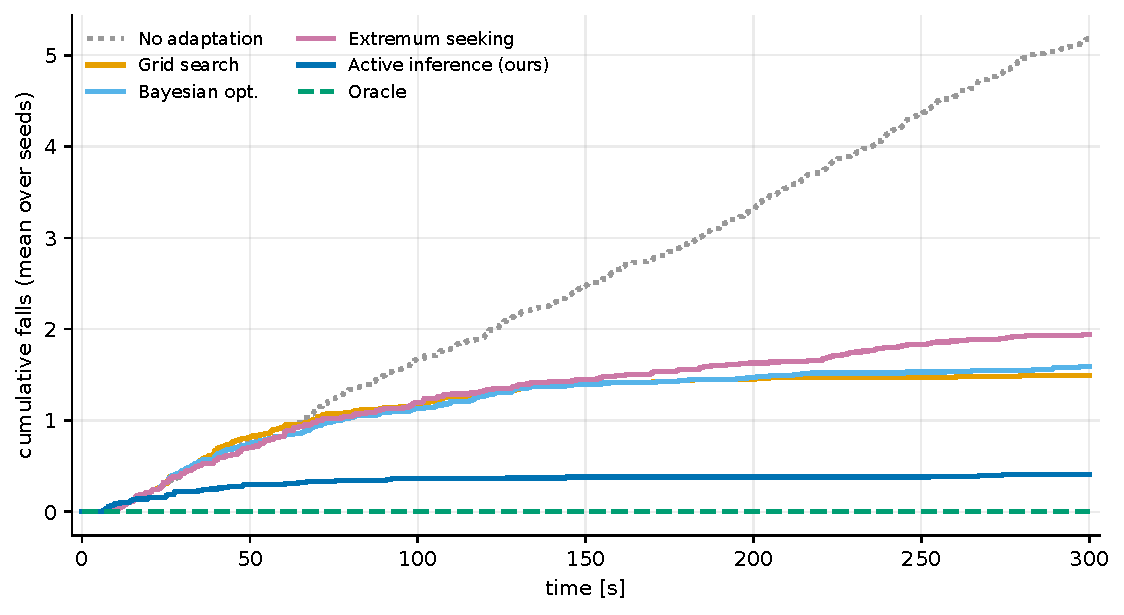
\includegraphics[width=\columnwidth]{payload_cumulative_falls.pdf}
\caption{Cumulative falls over a $300$\,s continual bout under the persistent payload shift (mean over one hundred seeds). Holding the incumbent gait accrues falls throughout. The three arms that must trial a candidate on the loaded robot (grid search, Bayesian optimization, extremum seeking) find a tolerant gait early but pay for the search first. The two arms that screen candidates against a memory of past falls, our agent and the safe Gaussian process ablation, fall far less and are indistinguishable from each other, which locates the benefit in the screening rather than in the unified objective.}
\label{fig:payload-falls}
\end{figure}

\begin{figure*}[t]
\centering
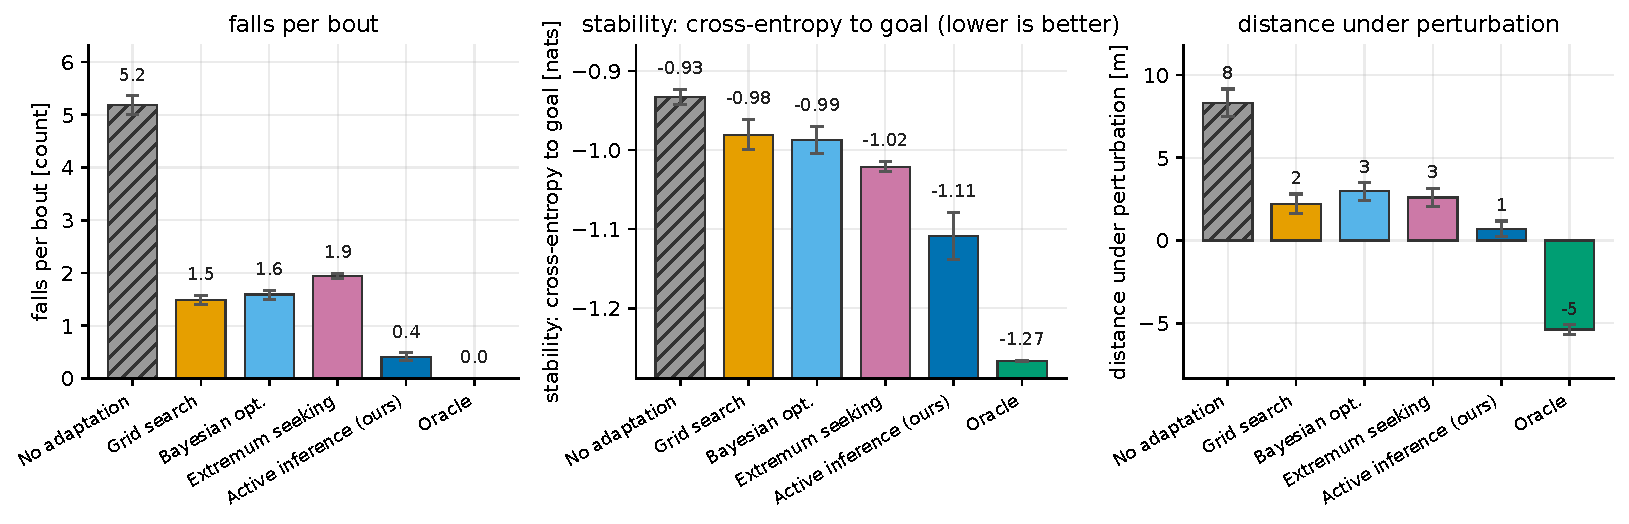
\includegraphics[width=0.92\textwidth]{payload_method_comparison.pdf}
\caption{Per-method outcome under the payload shift (mean over one hundred $300$\,s bouts): falls per bout, root-mean-square trunk tilt, and distance traveled while the payload is displaced. The adapting arms survive at a tilt comparable to the fixed gait but cover less ground, and the clairvoyant oracle is the most retrograde of all, which shows that the backward drift is a property of the gait parameterization rather than of the search.}
\label{fig:payload-comparison}
\end{figure*}

\begin{figure}[t]
\centering
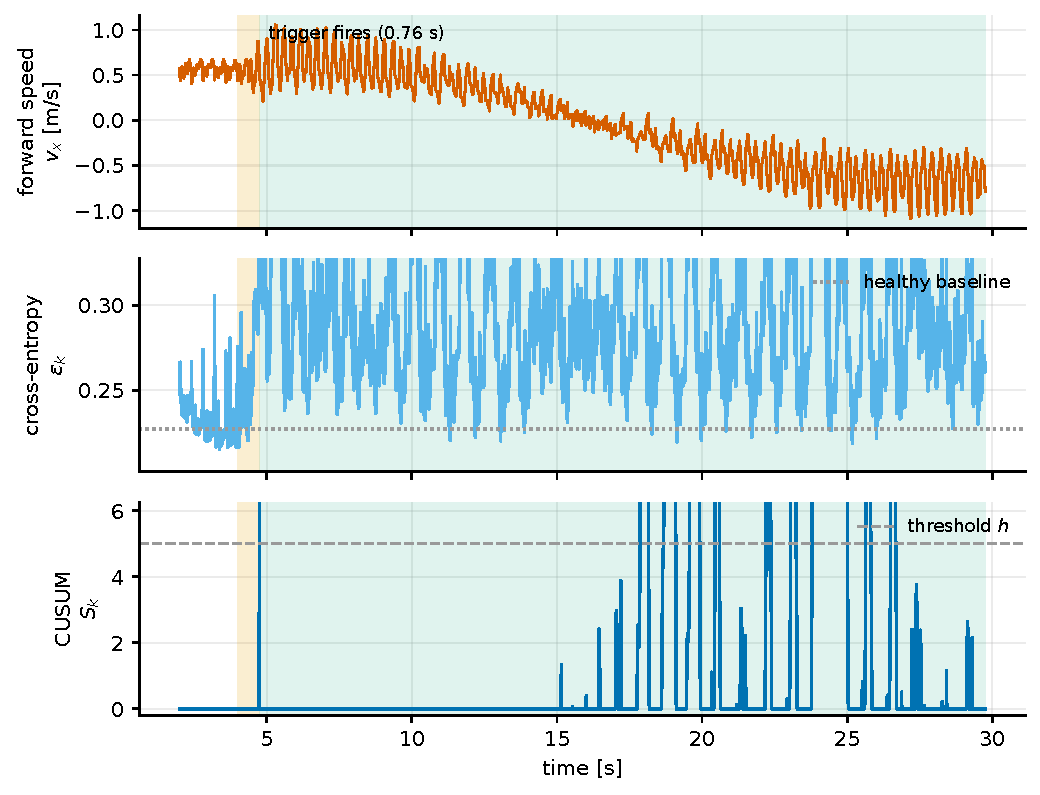
\includegraphics[width=\columnwidth]{payload_trigger.pdf}
\caption{The uprightness-only trigger over one payload shift (ours). \emph{Top:} forward speed, which the tolerant gait carries slowly backward under the load. \emph{Middle:} the attitude cross-entropy $\epsilon_k$ rests at its healthy baseline and rises when the shift tilts the trunk (shaded orange until the trigger fires, green once the proposed gait is active); it settles above baseline rather than returning to it. \emph{Bottom:} the CUSUM $S_k$ crosses its threshold $h$ within $0.76$\,s, is held at zero through the settle window, and re-crosses later in the bout without drawing a second adaptation, the monitor having latched for the event.}
\label{fig:payload-trigger}
\end{figure}

\subsection{Adapting to payload shifts}
\label{sec:exp-payload}

The scenario perturbs the mass distribution of the robot rather than its actuation.
The Laikago carries an $8$\,kg payload rigidly attached above its trunk, whose own mass is $10$\,kg, and at random intervals the payload shifts off the sagittal plane, $0.215$\,m laterally and $0.20$\,m to the rear, ramped over $1$\,s so that the change is a sustained bias rather than an impulse.
The offset then persists: once engaged it is held indefinitely, so the trunk bias compounds until the robot either falls or settles into a gait that tolerates the load.
This offset sits at the edge of recoverability.
Holding the incumbent gait $\theta^{\star}(\text{flat})$, the robot tips over on $85\%$ of shifts after a median of $33$\,s under the load, yet a re-tuned gait can stay upright indefinitely, so the perturbation rewards adaptation without being hopeless.
The bout is non-episodic and runs for $300$\,s: whenever the robot falls it is stood upright and the payload recentered, and after $2$ to $8$\,s the shift recurs.
A controller that never adapts therefore meets the same perturbation over and over, whereas one that finds a tolerant gait simply holds it and walks on, so an agent that remembers earlier outcomes should stop repeating the parameter choices that fell.

At each detected shift the agent proposes a gait by minimizing the Expected Free Energy of Eq.~\ref{eq:EFE} over its control map, favoring parameters whose predicted outputs lie near the goal while avoiding the regions its memory associates with falling.
It searches only the high-leverage subset $\{\gamma, \omega_{\text{swing}}, F_{\text{fast}}, K_{\text{stop}}, b\}$ of Eq.~\ref{eq:cpg-parameters}, and the memory persists across recurrences within the trial, so the map fills in as the shift repeats.
Adaptation is triggered by the cross-entropy criterion of Section~\ref{sec:trigger}: the MARX dynamics belief, updated online from the trunk outputs and the measured joint angles, drives the CUSUM once its one-step prediction departs the goal, and re-arms once the robot has recovered after each recenter.

Five further arms, each searching that same subset so that the comparison is head to head, place the agent among the alternatives.
Three are online optimizers that can judge a candidate gait only by running it: Latin-hypercube sampling (grid search), online Bayesian optimization, and extremum-seeking control, the classical model-free tuner, which dithers each parameter at a distinct frequency and demodulates the event score into a gradient estimate \cite{killingsworth2006extremum}.
Extremum seeking is the sharpest form of the difficulty, since even its exploratory dither must be executed on the already-loaded robot.
The fourth is an ablation that isolates the active inference machinery from safety-filtered search: a Gaussian process agent that screens candidates against the same memory of past falls, but driven by a hand-tuned prediction-error trigger rather than by the attitude marginal of the goal prior, and carrying no MARX belief of the body's dynamics.
The fifth is a clairvoyant oracle that jumps straight to a pre-fit tolerant gait, an upper anchor on any parameter switch.

Because a tolerant gait, once found, simply keeps walking, we run one hundred $300$\,s bouts per method and report the \emph{cumulative} falls that each accrues over a bout rather than a per-event rate (Fig.~\ref{fig:payload-falls}).
Holding the incumbent, the robot falls $5.18 \pm 0.18$ times per bout (mean $\pm$ s.e.m.), never adapting and tipping over on $85\%$ of recurrences.
Our agent instead falls only $0.41 \pm 0.08$ times, finding a tolerant gait after fewer than one fall on average and within the first $20$\,s, after which it holds that gait for the rest of the bout.
The three online optimizers fall in between, at $1.49 \pm 0.08$ (grid search), $1.59 \pm 0.09$ (Bayesian optimization) and $1.94 \pm 0.05$ (extremum seeking) falls per bout, each significantly worse than our agent (Mann-Whitney on per-seed fall counts, $p < 10^{-26}$).
They fall more because each can assess a candidate only by executing it on the already-shifted robot, where a poor candidate tips it over rather than merely scoring badly.
Extremum seeking is worst of the three, significantly worse than both grid search ($p \approx 6 \times 10^{-9}$) and Bayesian optimization ($p \approx 3 \times 10^{-6}$), even though its proposal is the cheapest to compute: its dither is by construction a perturbation applied to the loaded robot, so the exploration it needs in order to estimate a gradient is paid for in falls.
A clairvoyant oracle never falls, confirming that a recoverable gait exists within the searched subset.

The ablation qualifies what the active inference machinery contributes.
The safety-filtered Gaussian process agent, without the unified trigger and without the MARX belief, falls $0.48 \pm 0.08$ times per bout, statistically indistinguishable from our agent's $0.41 \pm 0.08$ ($p = 0.5$), and its fall accrual tracks ours closely throughout the bout (Fig.~\ref{fig:payload-falls}).
What separates the two groups is therefore whether a candidate is screened against a memory of past falls before it is walked on, not whether the trigger and the controller are read off a single goal prior.
The unified formulation should accordingly be read as an architectural simplification, one objective serving both roles at no cost in falls, rather than as the source of the improvement.
Where it does show a measurable edge is in promptness: the goal-prior trigger detects the shift in $0.93$\,s on average against $1.26$ to $1.38$\,s for the prediction-error monitors driving the other arms, with no false alarms in any arm.
Under the asynchronous protocol the gait proposal costs a median of one control step, since a tolerant gait is usually found before any Gaussian process fit is needed, rising to $1.74$\,s in the tail once the map is being fit.

The agent also stops re-tuning once a tolerant gait is in place, adapting exactly once per shift event across all one hundred bouts, so it does not chatter (Fig.~\ref{fig:payload-trigger}).
Two measurements qualify what produces that restraint.
The attitude prediction-error does not return to its healthy baseline: it settles about $17\%$ above the pre-shift level, and comes within $10\%$ of baseline in only $5\%$ of bouts, since a load held off-center is never quite free.
The accumulator does re-cross its threshold later in most bouts, and no second adaptation follows because the monitor latches for the remainder of the event.
The restraint is therefore a property of the event logic rather than evidence that the residual mismatch has vanished, and whether re-tuning on that residual would help is untested.

At this offset the tolerant gaits are more compromised than the fall counts alone convey (Fig.~\ref{fig:payload-comparison}).
Every adapting arm settles into a gait that walks slowly \emph{backward} under the load, at $-0.12$\,m/s for our agent and $-0.14$\,m/s for the three optimizers, against a $0.5$\,m/s forward target.
The clairvoyant oracle is the most retrograde of all at $-0.22$\,m/s, which is the informative part: the pre-fit gait that never falls is itself a backward one, so within this parameter subset no gait both tolerates the offset and makes forward progress.
The benefit here is thus strictly falls avoided, and reaching a gait that walks forward under the load is capped by the gait parameterization, as we discuss next.

%%%%%%%%%%%%%%%%%%%%%%%%%%%%%%%%%%%%%%%%%%%%%%%%%%%%%%%%%%%%%%%%%%%%%%%%%%%%%%%%
\section{DISCUSSION}
\label{sec:discussion}

Our results separate two aspects of online adaptation that are easily conflated: deciding \emph{when} to change the gait and deciding \emph{what} to change it to.
The prediction-error trigger resolves the first cheaply, reading uprightness rather than speed and re-arming to catch a recurring sequence, without a model of the perturbation.
The second is where the danger lies, since grid search, Bayesian optimization and extremum seeking can judge a candidate gait only by walking on it: on an already-perturbed robot a poor candidate does not merely score badly, it tips the robot over.
Extremum seeking makes the point most sharply, its dither being a deliberate perturbation of the loaded robot that costs more falls than the two search methods it is cheaper than.
Our agent instead screens each candidate against a learned map with an explicit memory of past falls, and it does so even though the CPG is already stabilized by the attitude controller, so the benefit is complementary to the reactive posture loop rather than a substitute for it.

The ablation narrows the claim.
A safety-filtered Gaussian process agent, given the same fall memory but neither the unified goal-prior trigger nor the dynamics belief, matches our agent's fall rate, so it is the screening that pays, not the unified objective.
We therefore read the unified formulation as an architectural economy, one goal prior specifying both when to act and what to do, removing a separately tuned detector at no cost in falls and detecting the shift somewhat sooner, rather than as a performance result.
Whether that economy earns more where a detector's threshold is harder to hand-tune remains untested.

Several limitations qualify these conclusions.
The evaluation is in simulation, over a single intrinsic perturbation and a modest number of recurrences, and the reference optima are computed offline.
More fundamentally, how much adaptation can recover is capped by the gait parameterization itself: under this payload offset no gait in the searched subset both tolerates the load and advances, the clairvoyant oracle itself walking backward at $0.22$\,m/s, so every online method settles somewhere between it and a standstill.
Staying upright and making progress are thus in tension here, and our agent, like the others, resolves that tension toward staying upright.
All arms pay the same price, so the comparison stays clean, but adapting \emph{without} surrendering the locomotion objective is left open, and likely requires a richer control representation rather than a better search within this one.
Validating on hardware, and across a wider range of perturbations, are natural next steps.

%%%%%%%%%%%%%%%%%%%%%%%%%%%%%%%%%%%%%%%%%%%%%%%%%%%%%%%%%%%%%%%%%%%%%%%%%%%%%%%%
\section{CONCLUSIONS}
\label{sec:conclusions}

We augmented a CPG of coupled Hopf oscillators with an attitude virtual model controller and studied when and how to re-tune its gait parameters online as the operating condition changes.
A prediction-error trigger decides when to adapt from a sustained loss of performance, and a unified active inference agent decides what to change by selecting parameters from a learned model of the body's response, with a persistent memory of past falls, rather than by physically trialing candidates.
On a shifting trunk payload, the agent learns within a single bout to stop selecting the gaits that fall, recovering without the destabilizing trials that grid search, Bayesian optimization and extremum seeking require.
An ablation attributes that gain to the memory-screened selection rather than to the unified objective, which matches it on falls while dispensing with a separately tuned detector.
How far this recovery generalizes, and how much the gait parameterization itself caps it, remain open.

%\addtolength{\textheight}{-3cm}  % This command serves to balance the column lengths
                                  % on the last page of the document manually. It shortens
                                  % the textheight of the last page by a suitable amount.
                                  % This command does not take effect until the next page
                                  % so it should come on the page before the last. Make
                                  % sure that you do not shorten the textheight too much.

%%%%%%%%%%%%%%%%%%%%%%%%%%%%%%%%%%%%%%%%%%%%%%%%%%%%%%%%%%%%%%%%%%%%%%%%%%%%%%%%
\bibliographystyle{IEEEtran}
\bibliography{references}

\end{document}
